\section{Theoretical Background of Neural Network}
    In this section, we're going to introduce the definition of neural networks, and its implementations in C as a library.
	\subsection{Neurons}
	Neurons are the fundamental part of the neural network, and they simulate the real neuron from organisms. To turn neuron into a math model, Scientists has given the specific definition and functions of neurons.   
	
	\begin{figure}[h]
	    \centering
	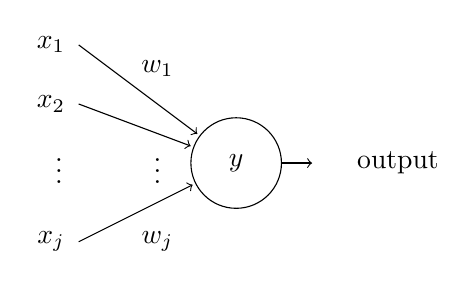
\begin{tikzpicture}[shorten >=1pt,->]
		\tikzstyle{unit}=[draw,shape=circle,minimum size=1.15cm]
 
		\node[unit](p) at (2,1){$y$};
		\node(dots) at (-0.25,1){\vdots};
		\node(dots2) at (1,1){\vdots};
		\node(w1) at (1.0,2.2){$w_1$};
		\node(wj) at (1.0,0){$w_j$};
 
		\draw (0,2.5) node[xshift=-10]{$x_1$} -- (p);
		\draw (0,1.75) node[xshift=-10]{$x_2$} --(p);
		\draw (0,0) node[xshift=-10]{$x_j$} -- (p);
		\draw (p) -- (3,1) node[xshift=30]{output};
% 		\draw (1.2,2.2) node[xshift=-10]{$w_1$};
	\end{tikzpicture}
	    \caption{Model of Neuron \cite{ref4}}
	    \label{fig:my_label}
	\end{figure}
	
	Since the actual neuron in real life sends electric signals only if the inputs have reached  specific conditions, we modeled it to be the \emph{threshold} of the neuron to activate and send a signal to neurons in the next layer. \emph{Weight} is then applied to every input to adjust the importance of each input, and the neuron only activates if the total sum of every input multiplied by its weight is greater than the threshold. The mathematical function of a neuron is given below:
	\begin{eqnarray}
  \mbox{output} & = & \left\{ \begin{array}{ll}
      0 & \mbox{if } \sum_j w_j x_j \leq \mbox{ threshold} \\
      1 & \mbox{if } \sum_j w_j x_j > \mbox{ threshold}
      \end{array} \right.
      \label{percep}
\end{eqnarray}
	Equation \ref{percep} shows one type of neurons: the perceptrons. However, in the modern model of neural networks, we use Sigmoid functions or Softmax functions with other approximating techniques to evaluate neuron outputs to imporve the accuracy of the trained model.   
	\subsection{Network of Neurons}
	As figure \ref{fig:nn-graph} shows, each neuron of the same layer is connected to every node of the next layer, therefore the output of this model can be transformed into matrix form:\\
	\paragraph{Matrixlization of Neuron Networks \cite{ref5}\\}
	Let $x$ inputs be numbered $i_1, i_2, \cdots i_x$, then matrix \textbf{I} is the matrix storing $1\times x$ elements of inputs in the same layer. 
	Each input neuron has its $y$ weights respectively points towards $y$ neurons of the next layer, then the total of input weight is represented by an $x\times y$ matrix \textbf{W}. Multiply \textbf{I} and \textbf{W} gets the inputs of the $y$  neuron in the next layer, stored in $ y\times 1$ matrix \textbf{H}. \\
	The same method can be done repetitively until the output layer is reached. 

 \begin{figure}[h!]
     \centering
    

\pagestyle{empty}

\def\layersep{2.5cm}

\begin{tikzpicture}[shorten >=1pt,->,draw=black!50, node distance=\layersep]
    \tikzstyle{every pin edge}=[<-,shorten <=1pt]
    \tikzstyle{neuron}=[circle,fill=black!25,minimum size=17pt,inner sep=0pt]
    \tikzstyle{input neuron}=[neuron, fill=green!50];
    \tikzstyle{output neuron}=[neuron, fill=red!50];
    \tikzstyle{hidden neuron}=[neuron, fill=blue!50];
    \tikzstyle{annot} = [text width=4em, text centered]

    % Draw the input layer nodes
    \foreach \name / \y in {1,...,4}
    % This is the same as writing \foreach \name / \y in {1/1,2/2,3/3,4/4}
        \node[input neuron, pin=left:Input \#\y] (I-\name) at (0,-\y) {};

    % Draw the hidden layer nodes
    \foreach \name / \y in {1,...,5}
        \path[yshift=0.5cm]
            node[hidden neuron] (H-\name) at (\layersep,-\y cm) {};

    % Draw the output layer node
    \node[output neuron,pin={[pin edge={->}]right:Output}, right of=H-3] (O) {};

    % Connect every node in the input layer with every node in the
    % hidden layer.
    \foreach \source in {1,...,4}
        \foreach \dest in {1,...,5}
            \path (I-\source) edge (H-\dest);

    % Connect every node in the hidden layer with the output layer
    \foreach \source in {1,...,5}
        \path (H-\source) edge (O);

    % Annotate the layers
    \node[annot,above of=H-1, node distance=1cm] (hl) {Hidden layer};
    \node[annot,left of=hl] {Input layer};
    \node[annot,right of=hl] {Output layer};
\end{tikzpicture}
% End of code

     \caption{An Example of Neural Network}
     \label{fig:nn-graph}
 \end{figure}

	